\documentclass[conference]{IEEEtran}
\IEEEoverridecommandlockouts
% The preceding line is only needed to identify funding in the first footnote. If that is unneeded, please comment it out.
\usepackage{cite}
\usepackage{amsmath,amssymb,amsfonts}
\usepackage{algorithmic}
\usepackage{graphicx}
\usepackage{textcomp}
\usepackage{xcolor}
\usepackage{url}
\def\BibTeX{{\rm B\kern-.05em{\sc i\kern-.025em b}\kern-.08em
    T\kern-.1667em\lower.7ex\hbox{E}\kern-.125emX}}

\begin{document}

\title{Practical Work I - Report\\
{\footnotesize \textsuperscript{}This report has been carried out for the ANADI Curricular Unit}
}

\author{
\IEEEauthorblockN{1\textsuperscript{st} Francisco Redol}
\IEEEauthorblockA{\textit{Instituto Politécnico do Porto} \\
\textit{ISEP - DEI}\\
Porto, Portugal \\
1201239@isep.ipp.pt}
\and

\IEEEauthorblockN{2\textsuperscript{nd} Mariana Lages}
\IEEEauthorblockA{\textit{Instituto Politécnico do Porto} \\
\textit{ISEP - DEI}\\
Porto, Portugal \\
1200902@isep.ipp.pt}
\and

\IEEEauthorblockN{3\textsuperscript{rd} Miguel Jordão}
\IEEEauthorblockA{\textit{Instituto Politécnico do Porto} \\
\textit{ISEP - DEI}\\
Porto, Portugal \\
1201487@isep.ipp.pt}
}

\maketitle

\begin{abstract}
On this report, we utilized R language features to support our affirmations and conclusions.
Themes such data analysis, data modeling and non/parametric tests were used on the data
from imported .csv files. 
\end{abstract}

\begin{IEEEkeywords}
regression, data analysis, data modeling, R language
\end{IEEEkeywords}

\section{Introduction}

Exploratory analysis is elected as the first step in a data analysis process, providing insights into a dataset's characteristics. By exploring and summarizing data through numerous statistical and graphical procedures, 
researchers can identify patterns, anomalies, and potential outliers, which can guide further analysis and hypothesis testing, along with formulating theories around a certain subject.
In this research, we will discuss key statistical aspects of that character, such as exploratory analysis, parametric and non-parametric tests, linear regression, and data modelling based on the provided datasets.
By giving an insight into these techniques and their applications, we aim to emphasise the importance of these backbone concepts while doing scientific research.
In the proposed assignment, there are three distinct datasets which will be thoroughly described, along with the steps to dissect these.

\subsection{Vehicles Dataset - Data Treatment}
The "Dados3.csv" dataset contains data about vehicle characteristics, such as acceleration, the number of cylinders in the engine, along with horsepower and the vehicle's weight.
Through exploratory analysis, given more context, it is possible to find hidden to the naked eye information, allowing a deeper understanding of a certain context.
For instance, a brand or a specific model.
\section{Exploratory Analysis - Vehicles}
Since the exercise requests to examine if there are significant differences in acceleration values between the three engine cylinder groups, 
it is pivotal to partition the acceleration values according to the number of cylinders. 
This is required because the proposed challenge questions if there are significant differences in the acceleration between vehicles, 
which leads to a concrete hypothesis test, allowing us to answer this question through the provided accelerations per cylinder.
So, two hypotheses were synthesized:

\begin{itemize}
    \item H0: There aren't significant differences between acceleration values according to the cylinder count;
    \item H1: There are significant differences between acceleration values between the distinct groups.
\end{itemize}

After formulating the two possible premises, we observe that the faced test is bilateral.
This is due to us facing an interest in solely finding out whether the mean acceleration of one group is higher or lower than the other one.\\

To prepare the data for the performed analysis, we first imported the dataset, which then was segregated into three distinct categories.
These are the different numbers of cylinder counts: 4, 6 and 8.\\

After setting up the required data, for the trial to be started, we needed to evaluate which kind of test could be performed on this population.
Starting with ANOVA, there are 6 exclusive steps which need to be accomplished.\\

First, is the dependent variable continuous? Because it varies according to the number of cylinders and takes infinite possibilities of values within a certain range, it is considered so.

Second, the independent variable (number of cylinders) has 3 groups of values, which complies with the two or plus variable groups.

Third, the observations are independent, considering that according to the essay, the number of cylinders is the key factor to consider in this variation.

Fourth, do the observations have significant outliers? To answer this question, a boxplot, which is a type of graphic that displays the median, quartiles, and outliers of the data was engendered.

\begin{figure}[htbp]
    \centering{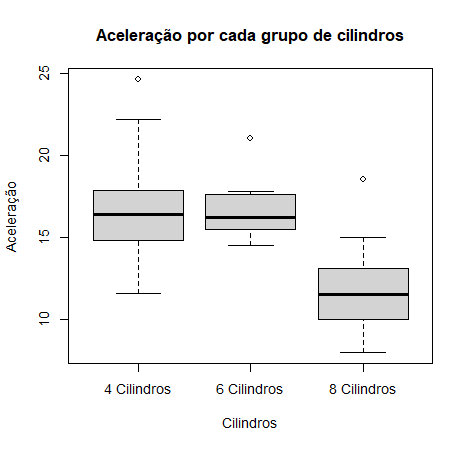
\includegraphics[width=5cm]{images/vehicles/boxplot.png}}
    \caption{Boxplot of the acceleration values according to the number of cylinders.}
    \label{vehicle_boxplot}
\end{figure}

At first sight, the results demonstrate that the 4-cylinder group has the highest median acceleration value (16.4), closely followed by the 6-cylinder group (16.2), 
which pulls a significant distance from the 8-cylinder engines acceleration (11.5). 
The interquartile range on 4 and 8-cylinders is much ampler than the 6-cylinders.
Its whiskers are also much more wide-ranging. 
Diving deeper into the quartiles analysis, for 4-cylinder powered vehicles, the quartile inferior limit is 10.2, with its superior limit around 22.4, close to the represented outlier. 
For the 6-cylinder, the inferior and superior limits were 12.3 and 20.8, respectively.
Lastly, on the 8-cylinder designed cars, 5.35 and 17.8.

After closely observing the boxplot it is confirmed that significant outliers exist, considering that acceleration is a continuous variable.
These are random points outside of the whiskers(highest and lowest observations within 1.5 times the interquartile range), particularly important when applied to a real-life scenario.
These could be explained by a vast number of variables, for instance, tyre pressure, which is outside of our scope.
Outliers are one of the most interesting/curious parts of a boxplot since they can reveal hidden causes.\\

However, 6-cylinder cars produce much more consistent results, while the remaining two have a wider spectre of traduced power.

Fifth, although we had a clear view that significant outliers existed, a Shapiro test, which verifies if a dependent variable is normally distributed was performed for each cylinder group.
For the 4-cylinder and 8-cylinder groups, the obtained significance level was 0.1056 and 0.2729, which could lead us to believe that homogeneity was achieved.
However, for the 6-cylinder group, the significance level peaked at 0.03628, which is inferior to the necessary 0.05, 
which obligates us to refute the theory which implies that the dependent variable is normally distributed.

With this conclusion taken, the possibility to use a parametric test such as One-Way ANOVA is ended. So, to test our original theory, we must use a 
non-parametric test. And, for that purpose, we reached the Kruskal-Wallis test.

On a Kruskal-Wallis test, if the predetermined significance level (which in this case is 0.05) is not met, the null hypothesis is rejected.
So, after fulfilling it, we could reach the conclusion that our p-value is 2.795e-11, leading to rejection H0, meaning that H1 is the accepted hypothesis, 
stating that there are significant differences between the cylinder groups.

\section{Linear Regression}

Linear regression is frequently used to forecast and analyze correlations between variables. On a practical side, it is commonly adopted in fields such as economics or engineering.
During the analysis of the dataset, four different plots were generated, which allowed us to verify the differences between the measured accelerations and the expected ones by the model.
The residuals sat around a median of -0.2788.

\subsection{Residuals vs Leverage}

The Residuals vs Leverage plot allows an analyst to verify if the provided dataset has many outliers which give insights to the researchers if they are being misled.
In this particular case, it shows a big concentration of data around the [-2,2] Residuals mark, 
with only a minority on other parts of the plot, which leads us to believe that the outliers are not influential on the interpreted result.

\begin{figure}[htbp]
    \centering{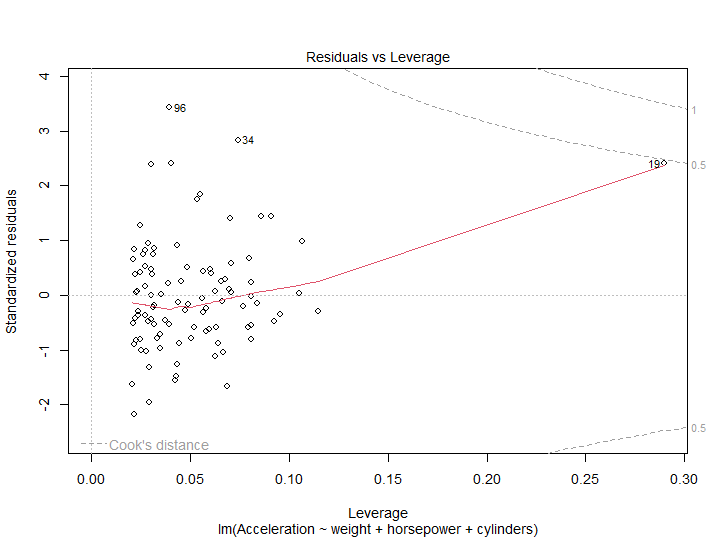
\includegraphics[width=5cm]{images/vehicles/residualsLeverage.png}}
    \caption{Graphic of the Residuals vs Leverage Regression Model}
    \label{residualsLeverage}
\end{figure}

\subsection{Residuals vs Fitted}

The Residuals vs Fitted plot allows an investigator to evaluate the provided data's quality and even possibly detect hidden patterns.
If the plot is properly adjusted between the two available variables, all the marked spots should be around 0. Analysing the given plot, even though the flagged values are around the 0 mark, 
we can observe a function slightly shaped like a very wide V, which makes us conclude that there may be some residue on certain groups, with the values being under/overestimated.
Ideally, the function should be as straight as possible, with the values spread around.

\begin{figure}[htbp]
    \centering{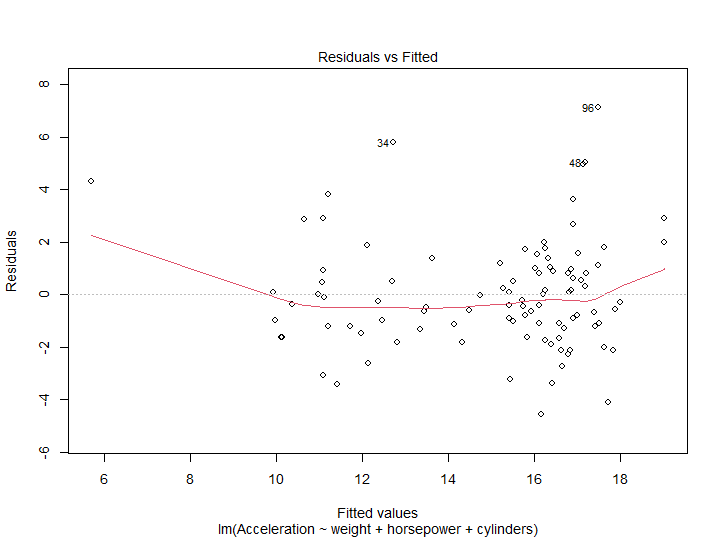
\includegraphics[width=5cm]{images/vehicles/residualsFitted.png}}
    \caption{Graphic of the Residuals vs Fitted Linear Regression Model}
    \label{residualsFitted}
\end{figure}

\subsection{Scale vs Location}

The Scale vs Location plot is another type of residual graphic used on linear regression.
Since this type of plot shows represents the square root of each value, for a graphic to be valuable (homoscedasticity), 
the points on the plot must be scattered horizontally around the line, which is the current case.

\begin{figure}[htbp]
    \centering{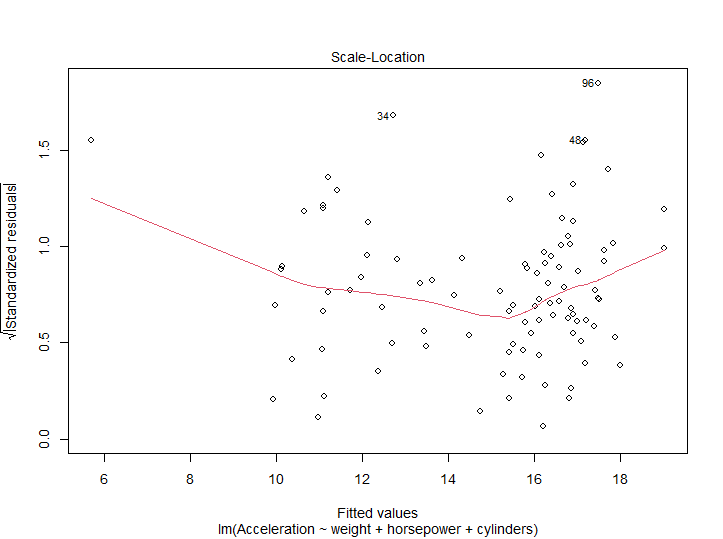
\includegraphics[width=5cm]{images/vehicles/scaleLocation.png}}
    \caption{Graphic of the Scale-Location Linear Regression Model}
    \label{scaleLocation}
\end{figure}

\subsection{Normal Q-Q}

Lastly, the Normal Q-Q Linear Regression plot allowed us to assess if the dataset was normally distributed.
Ideally, we want the points to be distributed closer to the line, which means that they would be normally distributed. 
Upon analysis, they are falling on an almost straight line, opposite to a bowed or S-pattern (which would represent skewness), this one is almost perfectly shaped, 
with a reduced number of outliers present.

\begin{figure}[htbp]
    \centering{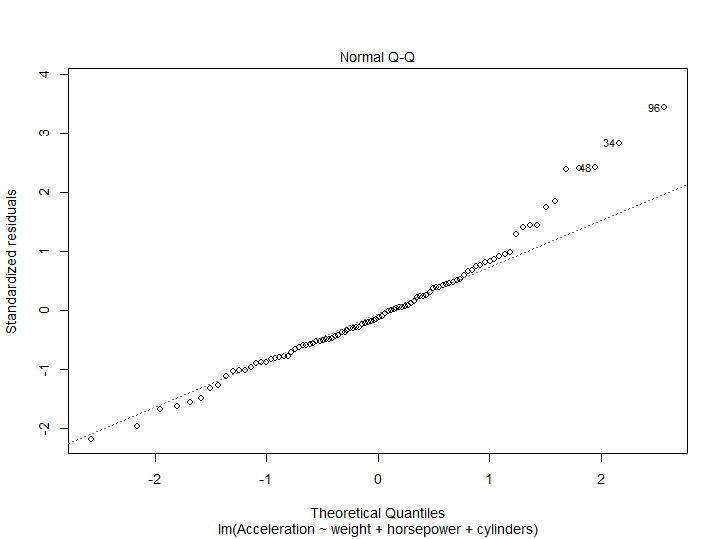
\includegraphics[width=5cm]{images/vehicles/normalQQ.png}}
    \caption{Graphic of the Normal Q-Q Linear Regression Model}
    \label{normalQQ}
\end{figure}

The positive feedback from the given plots allowed us to conclude that the dataset is certainly to be trustworthy.

\section{Prediction}

For the last exercise, it was requested to predict what would the acceleration of a car be if the engine had 4 cylinders, weighed 2950 kg and it had 100 horsepower. 
After performing a prediction, an acceleration value of 17.308, which belongs to 15\% 
between the 50\% below 16.4 and 75\% 17.85 is fitting into the provided graphics.

\section{Conclusion}

To put it concisely, the conclusion we extracted from the dataset is that when comparing the 3 groups, vehicles which have 4 cylinders have the higher acceleration, 
closely followed by 6 cylinders, with 8 cylinders vehicles bottoming out the list with the least acceleration.


\begin{thebibliography}{00}
\bibitem{b1} How to Use Q-Q Plots to Check Normality - Statology. (n.d.). Retrieved April 13, 2023, from \url{https://www.statology.org/q-q-plot-normality/}
\bibitem{b2} What is Considered a Good vs. Bad Residual Plot? - Statology. (n.d.). Retrieved April 13, 2023, from \url{https://www.statology.org/good-vs-bad-residual-plot/}
\bibitem{b3} How to Interpret a Scale-Location Plot (With Examples). (n.d.). Retrieved April 13, 2023, from \url{https://www.statology.org/scale-location-plot/}
\bibitem{b4} What is a Residuals vs. Leverage Plot? (Definition \& Example) - Statology. (n.d.). Retrieved April 13, 2023, from \url{"https://www.statology.org/residuals-vs-leverage-plot/}
\bibitem{b5} How to perform the Kruskal-Wallis test in R? | R-bloggers. Retrieved April 12, 2023, from \url{https://www.r-bloggers.com/2022/05/how-to-perform-the-kruskal-wallis-test-in-r/}
\bibitem{b6} A Complete Guide to Box Plots | Tutorial by Chartio. Retrieved April 12, 2023, from \url{https://chartio.com/learn/charts/box-plot-complete-guide/}
\end{thebibliography}
\vspace{12pt}
\color{red}
IEEE conference templates contain guidance text for composing and formatting conference papers. Please ensure that all template text is removed from your conference paper prior to submission to the conference. Failure to remove the template text from your paper may result in your paper not being published.

\end{document}
